%
% File naaclhlt2018.tex
%
%% Based on the style files for NAACL-HLT 2018, which were
%% Based on the style files for ACL-2015, with some improvements
%%  taken from the NAACL-2016 style
%% Based on the style files for ACL-2014, which were, in turn,
%% based on ACL-2013, ACL-2012, ACL-2011, ACL-2010, ACL-IJCNLP-2009,
%% EACL-2009, IJCNLP-2008...
%% Based on the style files for EACL 2006 by 
%%e.agirre@ehu.es or Sergi.Balari@uab.es
%% and that of ACL 08 by Joakim Nivre and Noah Smith

\documentclass[11pt,a4paper]{article}
\usepackage[hyperref]{acl2018}
\usepackage{times}
\usepackage{latexsym}
\usepackage{booktabs}
\usepackage{pgfplotstable}
\usepackage{url}
\usepackage{lipsum}
\usepackage{textcomp}

\usepackage{xspace}
\usepackage{multirow}

% My commands
\newcommand{\eqnref}[1]{Equation~\ref{#1}}
\newcommand{\figref}[1]{Figure~\ref{#1}}
\newcommand{\figsref}[2]{Figures~\ref{#1} and \ref{#2}}
\newcommand{\posciteauthor}[1]{\citeauthor{#1}'s}
\newcommand{\poscite}[1]{\citeauthor{#1}'s \citeyearpar{#1}}
\newcommand{\secref}[1]{Section~\ref{#1}}
\newcommand{\secsref}[2]{Sections~\ref{#1} and \ref{#2}}
\newcommand{\sentref}[1]{(\ref{#1})}
\newcommand{\tabref}[1]{Table~\ref{#1}}
\newcommand{\tabsref}[2]{Tables~\ref{#1} and \ref{#2}}

\newcommand{\dev}{\textsc{dev}\xspace}
\newcommand{\test}{\textsc{test}\xspace}
\newcommand{\skewed}{\textsc{skewed}\xspace}

\usepackage{array}
\newcolumntype{L}[1]{>{\raggedright\let\newline\\\arraybackslash\hspace{0pt}}m{#1}}
\newcolumntype{C}[1]{>{\centering\let\newline\\\arraybackslash\hspace{0pt}}m{#1}}
\newcolumntype{R}[1]{>{\raggedleft\let\newline\\\arraybackslash\hspace{0pt}}m{#1}}

%\setlength{\textfloatsep}{5pt}

\aclfinalcopy % Uncomment this line for the final submission
\def\aclpaperid{477} %  Enter the acl Paper ID here

%\setlength\titlebox{5cm}
% You can expand the titlebox if you need extra space
% to show all the authors. Please do not make the titlebox
% smaller than 5cm (the original size); we will check this
% in the camera-ready version and ask you to change it back.

\newcommand\BibTeX{B{\sc ib}\TeX}

\title{Leveraging distributed representations and lexico-syntactic
  fixedness for token-level prediction of the idiomaticity of English
  verb--noun combinations}

\author{Milton King \and Paul Cook \\
Faculty of Computer Science, University of New Brunswick\\
Fredericton, NB E3B 5A3 Canada\\
\tt{milton.king@unb.ca}, \tt{paul.cook@unb.ca}}
%% \author{Milton King \\
%%   University of New Brunswick\\ Fredericton, NB\\
%%   {\tt milton.king@unb.ca} \\}

\date{}

%% TODO: Acknowledge that Salton et al. considered additional SVM kernels
%% and did better than with a linear one. I think that's OK though,
%% because we're interested in what happens to the different models under
%% some learning algorithm, so that shouldn't be a big deal.

%% TODO: Motivate why we used the particular word2vec settings that we did

\begin{document}
\maketitle

\begin{abstract}
Verb--noun combinations (VNCs) --- e.g., \emph{blow the whistle},
\emph{hit the roof}, and \emph{see stars} --- are a common type of
English idiom that are ambiguous with literal usages. In this paper we
propose and evaluate models for classifying VNC usages as idiomatic or
literal, based on a variety of approaches to forming distributed
%% representations. Our experimental results show that a simple model
representations. Our results show that a model
based on averaging word embeddings performs on par with, or better
than,
%% improves over 
a previously-proposed approach based on skip-thoughts. Idiomatic
usages of VNCs are known to exhibit lexico-syntactic fixedness. We
further incorporate this information into our models, demonstrating
that this rich linguistic knowledge is complementary to the
information carried by distributed representations.

%% An idiomatic occurrence of a multiword expression (MWE) has a
%% different meaning than its literal counterpart and therefore raises
%% issues with applications such as machine translation. 

%% Idiom token classification involves determining if an MWE is idiomatic
%% or literal. 

%% We apply a variety of embedding-based models in a supervised setup to
%% an idiom token classification task that works with verb-noun
%% combination (VNCs). 

%% We further improve the performance of models by determining if the
%% combination of words are in a canonical form, which is a
%% lexico-syntactic pattern that idiomatic usages of a VNC tend to occur
%% in. 

%% We discover that averaging word2vec embeddings as input to a
%% support vector machine achieves the highest accuracy on both of our
%% datasets.

\end{abstract}

\section{Introduction}



%% Define MWEs and semantic idiomaticity

%% Define VNCs; explain their token-level ambiguity; define the task of
%% MWE identification

Multiword expressions (MWEs) are combinations of multiple words that
exhibit some degree of idiomaticity
\citep{Baldwin:Kim:2009}. Verb--noun combinations (VNCs), consisting
of a verb with a noun in its direct object position, are a common type
of semantically-idiomatic MWE in English and cross-lingually
\citep{Fazly2009}. Many VNCs are ambiguous between MWEs and literal
combinations, as in the following examples of \emph{see stars}, in
which \ref{ex:idm} is an idiomatic usage (i.e., an MWE), while
\ref{ex:lit} is a literal combination.\footnote{These examples, and
  idiomaticity judgements, are taken from the VNC-Tokens dataset
  \citep{Cook2008}.}

\begin{enumerate}
\item Hereford United were \underline{seeing stars} at Gillingham
  after letting in 2 early goals \label{ex:idm}

\item Look into the night sky to \underline{see} the
  \underline{stars} \label{ex:lit}
\end{enumerate}

\noindent
MWE identification is the task of automatically determining which word
combinations at the token-level form MWEs \citep{Baldwin:Kim:2009},
and must be able to make such distinctions. This is particularly
important for applications such as machine translation
\citep{Sag2002}, where the appropriate meaning of word combinations in
context must be preserved for accurate translation.

%% This approach, referred to as CForm, is a strong,
%% linguistically-informed, unsupervised baseline for VNC
%% identification.

In this paper, following prior work
\citep[e.g.,][]{salton-ross-kelleher}, we frame token-level
identification of VNCs as a supervised binary classification problem,
i.e., idiomatic vs.\ literal. We consider a range of approaches to
forming distributed representations of the context in which a VNC
occurs, including word embeddings \citep{mikolov+:2013b}, word
embeddings tailored to representing sentences
\citep{kenter-borisov-derijke}, and skip-thoughts sentence embeddings
\cite{Kiros+:2015}.  We then train a support vector machine (SVM) on
these representations to classify unseen VNC instances. Surprisingly,
we find that an approach based on representing sentences as the
average of their word embeddings performs comparably to, or better
than,
%% best, and in particular outperforms
the skip-thoughts based approach previously proposed by
\newcite{salton-ross-kelleher}.

VNCs exhibit lexico-syntactic fixedness. For example, the idiomatic
interpretation in example \ref{ex:idm} above is typically only
accessible when the verb \emph{see} has active voice, the determiner
is null, and the noun \emph{star} is in plural form, as in \emph{see
  stars} or \emph{seeing stars}.  Usages with a determiner (as in
example \ref{ex:lit}), a singular noun (e.g., \emph{see a star}), or
passive voice (e.g., \emph{stars were seen}) typically only have the
literal interpretation.

%% Maybe we can avoid saying this here
%% Drawing on observations about the lexico-syntactic fixedness of VNCs,
%% \newcite{Fazly2009} proposed an unsupervised statistical method to
%% identify a VNC's canonical form, i.e., the lexico-syntactic form in
%% which the idiomatic interpretation is accessible --- \emph{see stars}
%% in the example above. They then showed that idiomatic usages of a VNC
%% tend to correspond to its canonical form.

%% TODO: Mention this in a footnote somewhere
%% We further consider embedding-based models for document classification
%% \citep{joulin-EtAl} and a classifier based on a convolutional neural
%% network \citep{kim:2014}.

In this paper we further incorporate knowledge of the lexico-syntactic
fixedness of VNCs --- automatically acquired from corpora using the
method of \newcite{Fazly2009} --- into our various embedding-based
approaches. Our experimental results show that this leads to
substantial improvements, indicating that this rich linguistic
knowledge is complementary to that available in distributed
representations.



%% Intro for NAACL

%% Multiword expressions (MWEs) are combinations of multiple words that
%% exhibit some degree of idiomaticity \citep{Baldwin:Kim:2009}. One
%% common form of idiomaticity is \emph{semantic idiomaticity}, whereby
%% the meaning of an expression is not transparent based on the meanings
%% of its component words. For example, the meaning of a brief,
%% unrepeatable success for the expression \emph{flash in the pan} is not
%% transparent from its component words. Moreover, many combinations are
%% ambiguous at the token level between MWEs (exhibiting semantic
%% idiomaticity) and similar-on-the-surface literal combinations. For
%% example, \emph{red flag} can be used as an MWE to mean a warning, but
%% can also be used as a literal combination (non-MWE) referring to a
%% flag that is red. Work on MWE identification
%% \citep[e.g.,][]{Birke2006,Fothergill:Baldwin:2012,salton-ross-kelleher}
%% aims to automatically determine which word combinations at the
%% token-level form MWEs, and must be able to make such
%% distinctions. This is particularly important for applications such as
%% machine translation \citep{Sag2002}, where the meaning word
%% combinations must be preserved to form an accurate translation

%% Verb--noun combinations (VNCs), consisting of a verb with a noun in
%% its direct object position, are a common type of
%% semantically-idiomatic MWE in English and cross-lingually
%% \citep{Fazly2009}. Many VNCs are ambiguous between MWEs and literal
%% combinations, as in the following two examples of \emph{see stars}, in
%% which the first is an idiomatic usage (i.e., an MWE), while the second
%% is a literal combination.\footnote{These examples, and idiomaticity
%%   judgements, are taken from the VNC-Tokens dataset \citep{Cook2008}.}


%% \begin{enumerate}
%% \item Hereford United were \underline{seeing stars} at Gillingham
%%   after letting in 2 early goals

%% \item Look into the night sky to \underline{see} the
%%   \underline{stars}
%% \end{enumerate}

%% \noindent
%% VNCs exhibit lexico-syntactic fixedness. For example, the idiomatic
%% interpretation above is typically only accessible when the verb
%% \emph{see} has active voice, the determiner is null, and the noun
%% \emph{star} is in plural form, as in \emph{see stars} or \emph{seeing
%%   stars}.  For usages with a determiner or singular noun (e.g.,
%% \emph{see a star}) or passive voice (e.g., \emph{stars were seen})
%% typically only the literal interpretation is accessible.

%% Previous work has framed the task of token-level identification of
%% VNCs as a binary classification problem, i.e., idiomatic vs. literal
%% \citep[e.g.,][]{Fazly2009,salton-ross-kelleher}. \newcite{salton-ross-kelleher}
%% applied skip-thoughts \cite{Kiros+:2015} --- an encoder--decoder model
%% that can be viewed as a sentence-level counterpart to the word2vec
%% \citep{mikolov+:2013b} skip-gram model --- to form distributed
%% representations of sentences containing VNCs. They then trained a
%% support vector machine (SVM) on these representations to classify new
%% VNC instances.

%% In this paper, we use a similar experimental setup to
%% \newcite{salton-ross-kelleher}, i.e, supervised approaches to binary
%% classification; however, we consider a wider range of approaches to
%% representing VNC instances. Specifically we consider the use of word
%% embeddings \citep{mikolov+:2013b} and word embeddings tailored to
%% representing sentences \citep{kenter-borisov-derijke}. We further
%% consider embedding-based models for document classification
%% \citep{joulin-EtAl} and a classifier based on a convolutional neural
%% network \citep{kim:2014}. Surprisingly, we find that an approach based
%% on representing sentences as the average of their word embeddings and
%% an SVM performs best, and in particular outperforms the skip-thoughts
%% based approach of \citeauthor{salton-ross-kelleher}

%% Drawing on observations about the lexico-syntactic fixedness of VNCs,
%% \newcite{Fazly2009} proposed an unsupervised statistical method to
%% identify a VNC's canonical lexico-syntactic form (i.e., the
%% lexico-syntactic form in which the idiomatic interpretation is
%% accessible --- \emph{see stars} in the example above). They then
%% showed that idiomatic usages of a VNC tend to correspond to its
%% canonical form. This approach, referred to as CForm, is a strong,
%% linguistically-informed, unsupervised baseline for VNC identification.

%% %% TODO Could improve strength of results based on a hypothesis
%% %% test. MacNemar's test could be applied.

%% In this paper we further incorporate knowledge of whether a VNC
%% instance occurs in its canonical form into our various embedding-based
%% approaches. Our experimental results show that this leads to
%% substantial improvements, indicating that the rich linguistic
%% knowledge captured by these canonical forms is complementary to that
%% available in distributed representations.


%% Old bits
%% Usages of an MWE can be either idiomatic or literal. An idiomatic
%% instance of an MWE exhibits a semantic meaning that is not
%% distinguishable by analyzing its components. For an example, the
%% phrase \textit{kick the bucket} can represent someone has died when
%% occurring as idiomatic or that someone hit a physical bucket with
%% their foot when occurring as a literal. The difference in meaning can
%% cause issues in applications such as machine translation
%% \citep{Sag2002}, where the meaning of words need to be preserved to
%% form an accurate translation. Idiom token classification is used to
%% distinguish if an instance of an MWE is idiomatic or literal, which
%% can assist in determining the meaning of the MWE. In this paper, we
%% will be applying different embedding-based models to an idiom
%% classification task which contains instances of VNC's. VNC's are MWE's
%% that contain a verb and a noun such as \textit{see stars}.

%% In this paper, we first discuss other work that is related to idiom
%% token classification and MWE identification in Section
%% \ref{related}. We then discuss our idiom classification tack is detail
%% in Section \ref{idiom}. The embedding models that are used are
%% described in Section \ref{models}. We discuss the dataset and
%% evaluation metrics that we use along with how the embedding models are
%% used in Sections \ref{dataset}, \ref{eval}, and \ref{applied},
%% respectively. We show and analyze our results in Section \ref{results}
%% with our conclusion and insight into further experiments in Section
%% \ref{conclusion}, and \ref{future}, respectively.

%% Idiom token classification involves labeling the instance of a VNC as
%% being an idiom or literal. We apply a variety of models to an idiom
%% token classification task. These models include the use of generic
%% word embeddings \citep{mikolov+:2013a}, word embeddings specifically
%% designed for representing a sentence \citep{kenter-borisov-derijke},
%% sentence embeddings \citep{Kiros+:2015}, an embedding-based models
%% specifically trained for a single task \citep{joulin-EtAl}, and
%% convolutional neural networks
%% \citep{kim:2014}. \cite{salton-ross-kelleher} applied a sentence
%% embedding model --known as skip-thoughts \citep{Kiros+:2015}-- to
%% instances from the dataset that we work with, while
%% \cite{gharbieh2016word} applied word2vec's word embeddings.


\section{Related work} \label{related}

%% Compositionality prediction --- i.e., determining the extent to which
%% the meaning of an MWE type is transparent based on the meanings of its
%% component words \citep[e.g.,][]{Reddy+:2011,Salehi+:2015} --- and
%% multiword expression extraction --- i.e., finding all MWE types that
%% are present in a given corpus \citep[e.g.,][]{Church1990,Lin1999} ---
%% are important type-level tasks that have been widely examined in
%% computational work on MWEs. In contrast, this paper focuses on MWE
%% identification, a token-level prediction task.

%% TODO: First two paragraphs could be trimmed

Much research on MWE identification has focused on specific kinds of
MWEs \citep[e.g.,][]{Patrick2005, Uchiyama2005}, including English
VNCs \citep[e.g.,][]{Fazly2009,salton-ross-kelleher}, although some
recent work has considered the identification of a broad range of
kinds of MWEs
\citep[e.g.,][]{Schneider+:2014,Brooke+:2014,savary-EtAl:2017:MWE2017}.

Work on MWE identification has leveraged rich linguistic knowledge of
the constructions under consideration
\citep[e.g.,][]{Fazly2009,Fothergill:Baldwin:2012}, treated literal
and idiomatic as two senses of an expression and applied approaches
similar to word-sense disambiguation
\citep[e.g.,][]{Birke2006,Hashimoto:Kawahara:2008}, incorporated topic
models \citep[e.g.,][]{Li+:2010}, and made use of distributed
representations of words \citep{gharbieh+:2016}.
%% and sentences \citep{salton-ross-kelleher}.

%% The most closely related work to ours is
%% \newcite{salton-ross-kelleher}. They represent token instances of VNCs

In the most closely related work to ours,
\newcite{salton-ross-kelleher} represent token instances of VNCs by
embedding the sentence that they occur in using skip-thoughts
\citep{Kiros+:2015} --- an encoder--decoder model that can be viewed
as a sentence-level counterpart to the word2vec \citep{mikolov+:2013b}
skip-gram model. During training the target sentence is encoded using
a recurrent neural network, and is used to predict the previous and
next sentences. \citeauthor{salton-ross-kelleher} then use these
sentence embeddings, representing VNC token instances, as features in
a supervised classifier.  We treat this skip-thoughts based approach
as a strong baseline to compare against.

%% TODO: Make sure we make it clear we are comparing against their
%% ``general'' setup in the description of the dataset.

%% \newcite{salton-ross-kelleher} consider two different experimental
%% setups --- ``per expression'' and ``general''. In the per expression
%% setup, a classifier is trained on token instances of only one VNC
%% expression, and is then used to classify further instances of that
%% same VNC type; \citeauthor{salton-ross-kelleher} limited their per
%% expression experiments to just four VNCs: \emph{blow whistle},
%% \emph{lose head}, \emph{make scene}, and \emph{take heart}. In the
%% general setup, the classifier is trained on instances of many VNC
%% types, and is then used to classify further instances of these
%% expressions. In this paper we use a similar experimental setup to the
%% general setup of \citeauthor{salton-ross-kelleher} and evaluate on the
%% same dataset they used. We treat their skip-thoughts based approach
%% using a SVM classifier as a strong baseline to compare against.



%% : Possibly move these details into later section
%% \cite{salton-ross-kelleher} generate a training a testing set by
%% preserving a distribution over a number of idiomatic and literal
%% usages of an VNC. Each VNC will be in both the training and testing
%% allowing a model to see each VNC that is in the testing while training
%% on the training set.

%% For both the per expression setup and the general setup, they compared
%% the performance of three different types of SVM's including a linear
%% SVM, a linear SVM that used stochastic gradient descent, and an SVM
%% with a polynomial kernel. They also used a k-nearest neighbour
%% classifier for the per expression setup as well, where they evaluated
%% their model with different values for k. The per expression setup was
%% only used on four VNC's --blow\_whistle, lose\_head, make\_scene, and
%% take\_heart. They averaged the recall, precision, and f1-score over
%% ten runs. The linear SVM and the SVM with a polynomial kernel achieved
%% the highest f1-score overall in the general setup. The SVM with
%% polynomial kernel achieved the highest f1-score on most of the VNC's
%% in the per expression setup.

%% We also draw heavily on \newcite{Fazly2009}. 

\newcite{Fazly2009} formed a set of eleven lexico-syntactic patterns
for VNC instances capturing the voice of the verb (active or passive),
determiner (e.g., \emph{a}, \emph{the}), and number of the noun
(singular or plural).  They then determine the canonical form,
$C(v,n)$, for a given VNC as follows:\footnote{In a small number of
  cases a VNC is found to have a small number of canonical forms, as
  opposed to just one.}
\begin{equation}
C(v,n) = \{ pt_k \in P | z(v,n,pt_k) > T_z \}
\end{equation}
\noindent
where $P$ is the set of patterns, $T_z$ is a predetermined threshold,
which is set to 1, and $z(v,n,pt_k)$ is calculated as follows:
\begin{equation}
z(v,n,pt_k)= \frac{f(v,n,pt_k)-\overline{f}}{s}
\end{equation}
\noindent
where $f(\cdot)$ is the frequency of a VNC occurring in a given
pattern in a corpus,\footnote{\newcite{Fazly2009} used the British
  National Corpus \citep{Burnard2000}.} and $\overline{f}$ and $s$ are
the mean and standard deviations for all patterns for the given VNC,
respectively.

\newcite{Fazly2009} showed that idiomatic usages of a VNC tend to
occur in that expression's canonical form, while literal usages do
not. This approach provides a strong, linguistically-informed,
unsupervised baseline, referred to as CForm, for predicting whether
VNC instances are idiomatic or literal. In this paper we incorporate
knowledge of canonical forms into embedding-based approaches to VNC
token classification, and show that this linguistic knowledge can be
leveraged to improve such approaches.

%% TODO: Could possibly drop the last sentence above; it's mentioned
%% in the introduction


%% Old bits
%% The z-score works on the idea that a VNC will occur in its idiom form
%% more often than its literal. They set $T_z$ to $1$, which we do as
%% well for our experiments.

%% They label each VNC instance as belonging to one of these patterns.

%% They then determine which patterns that a particular VNC is often
%% labeled as idiomatic while occurring in these patterns.

%% This is known as a canonical form and the set of canonical forms for a
%% single VNC is calculated as $C(v,n) = \{ pt_k \in P | z(v,n,pt_k) >
%% T_z \}$, where $P$ is the set of patterns, $T_z$ is a predetermined
%% threshold and $z(v,n,pt_k)$ is calculated as $z(v,n,pt_k)=
%% \frac{f(v,n,pt_k)-\overline{f}}{s}$, where $f(\cdot)$ is the frequency
%% of a VNC occurring in a given pattern and $\overline{f}$ and $s$ are
%% the mean and standard deviations for all patterns for the given VNC,
%% respectively. The z-score works on the idea that a VNC will occur in
%% its idiom form more often than its literal. They set $T_z$ to $1$,
%% which we do as well for our experiments.


%% \begin{figure}
%% 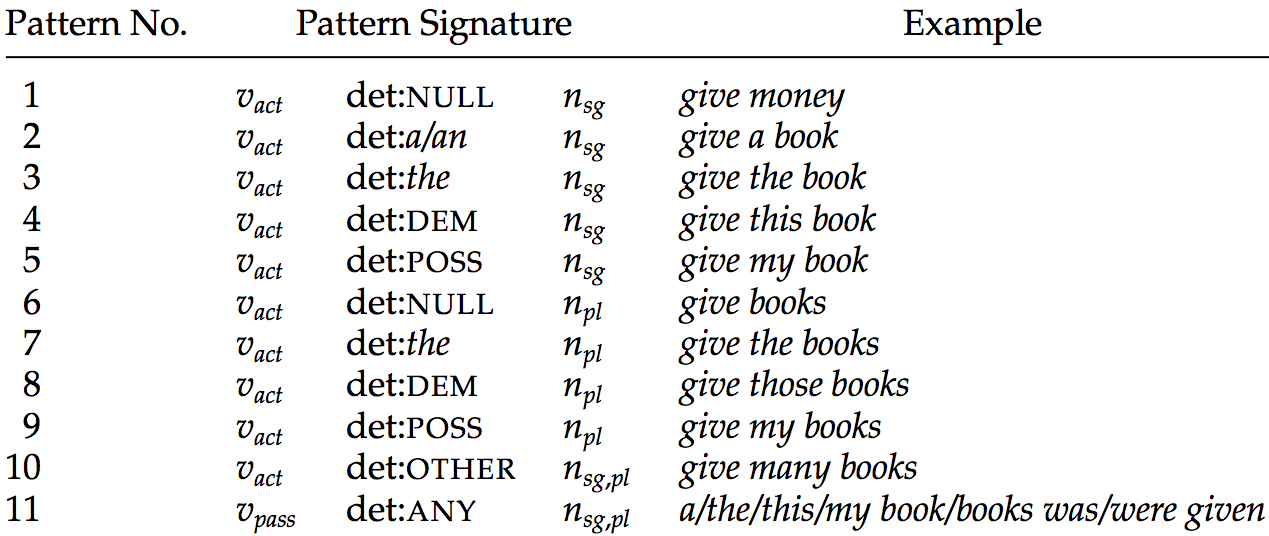
\includegraphics[width=\linewidth]{./patterns}
%%   \caption{Lexico-syntactic patterns for VNCs, taken from
%%     \newcite{Fazly2009}.}
%%   \label{fig:patterns}
%% \end{figure}









%% Old bits
%% \cite{Sag2002} discusses many types of MWE's and explain how they can
%% cause issues for applications such as machine translation. For
%% example, the phrase \textit{kick the bucket} can be translated to
%% another language while preserving either the meaning of \textit{death}
%% or \textit{hitting a bucket with one's foot}. Accurately capturing the
%% meaning of words, such as MWE's, can also benefit other tasks such as
%% usage similarity \citep{LuiBaldwin2012}, word sense induction
%% \cite{Manandhar+:2010}, and information retrieval
%% \citep{Schütze95informationretrieval}. Usage similarity involves
%% determining the similarity of two usages of the same word in two
%% different contexts. The effects of an MWE being idiomatic or literal
%% can be seen if we wanted to see how similar the sentence \textit{I'd
%%   like to see the stars through a telescope} is to the two sentences
%% in Figure \ref{examples}. The idiomatic instance captures the meaning
%% of being disoriented or dizzy and would have a low similarity with the
%% given sentence but, the literal instance in Figure \ref{examples}
%% captures the meaning of seeing bright physical objects in outer space,
%% which would have a higher similarity with the given sentence. Word
%% sense induction is similar to usage similarity, except in this task
%% all instances of a word are clustered together based on the sense that
%% they exhibit in their context. A sense is the meaning that a word
%% takes on in context. Given the same three examples, we would want our
%% model to cluster the given sentence and the literal example sentence
%% together and map the idiom sentence to another cluster. If the
%% idiomatic nature is not detected then there is a chance that all three
%% sentences could be clustered together and the senses of the MWE would
%% not be preserved. Information retrieval involves returning the most
%% relevant documents for a query. The effects of idiomatic usages can be
%% seen if we wanted to search about when someone \textit{died}, then we
%% would want all documents that used the MWE \textit{kick the bucket} as
%% an idiom and not as a literal interpretation.

%% \begin{figure}[h]
%% (Idiom) I\textquotesingle d see a lot more stars when Carmen hit me\\
%% (Literal) Look into the night sky to see the stars
%%   \caption{Examples of an idiom and a literal instance of the VNC $see stars$ with their label in parenthesis.}
%%   \label{examples}
%% \end{figure}


%% PARSEME is an organization that releases shared tasks that focus on
%% parsing text containing
%% MWE's\footnote{\url{https://typo.uni-konstanz.de/parseme/}}. In 2017,
%% they released a shared task that involves automatically identifying
%% verbal MWE's (VWME's) \citep{savary-EtAl:2017:MWE2017}. This task
%% involved text in eighteen different languages and required models to
%% identify VMWE's in a sentence. \cite{maldonado-EtAl:2017:MWE2017}
%% approached this task with a conditional random fields model
%% (CRF). CRF's are a statistical model used to predict a sequence of
%% labels. The features that they used include words, lemmas, and POS. If
%% there is more syntactic information available they also include a
%% token's head's word, head's lemma, head's POS, and the dependency
%% between the token and the head. They made a version of their model
%% where they have their CRF output ten different sequences, which they
%% extract features from to form ten different vectors to then be input
%% for a regression algorithm. The regression algorithm would select the
%% most likely sequence. The features that they used for this version
%% include words co-occuring with the MWE in the Europarl
%% corpus\footnote{\url{http://www.statmt.org/europarl/}}, comparing
%% MWE's with only one word of the full MWE with the full MWE, MWE's with
%% one less word than the full MWE, and comparing other MWEs found in the
%% 10 sequences. \cite{borocs-EtAl:2017:MWE2017} also approached this
%% task with a CRF using similar features but they label the head word
%% first and then the tail words.
%% \cite{nerima-foufi-wehrli:2017:MWE2017} attempted this task with a
%% constituent parser. Their model uses the output of their parser along
%% with a set of rules to identify a VMWE. Similarly,
%% \cite{alsaied-constant-candito:2017:MWE2017} applied a transition
%% parser that uses an SVM to determine the transitions and an MWE is
%% identified when the SVM predicts a specific transition.
 
%Discuss type of embeddings
%% Embeddings are vector representations of words, which are usually
%% generated by artificial neural networks. Embeddings can represent a
%% character \citep{NIPS2015_5782}, a word \citep{mikolov+:2013a}, a
%% sense \citep{neelakantan2015efficient}, a sentence
%% \citep{Kiros+:2015}, the context of a word
%% \citep{melamud2016context2vec}, and a paragraph
%% \citep{Le:Mikolov:2014}. Embeddings have been responsible for
%% state-of-the-art performances in many text classification tasks. More
%% importantly, they have performed well on idiom classification tasks
%% \citep{salton-ross-kelleher, gharbieh2016word}. This supports our
%% reasoning for using embedding models on our idiom classification task.



%Waseem paper
%% The closest work to ours is the work done in \cite{gharbieh2016word},
%% where they also apply word embeddings to identify idiomaticity of an
%% VNC. They represent an instance of an VNC by first averaging the two
%% word embeddings for the lemmas of the two components in the VNC to
%% form the vector $t$. They then average the embeddings of the context
%% words within a predetermined window separately for the verb and noun
%% giving the vectors $v$ and $n$, respectively. The vectors $v$ and $n$
%% are then averaged forming $vn$. They generate their final feature
%% vector by subtracting $vn$ from $t$ and concatenating it with a binary
%% feature representing if the instances is in a canonical form. They
%% proposed a supervised and unsupervised model, which both use the same
%% feature vector that was described above. Their supervised model uses
%% an SVM for classification. Their unsupervised model uses k-means
%% clustering to form clusters and they label the instances in a cluster
%% idiomatic if the majority of them are in a canonical form.





%% \section{Idiom token classification} \label{idiom}

%% Old section 3: content moved to intro and RW

%% Idiom token classification involves labeling the instance of a VNC as
%% being an idiom or literal. We apply a variety of models to an idiom
%% token classification task. These models include the use of generic
%% word embeddings \citep{mikolov+:2013a}, word embeddings specifically
%% designed for representing a sentence \citep{kenter-borisov-derijke},
%% sentence embeddings \citep{Kiros+:2015}, an embedding-based models
%% specifically trained for a single task \citep{joulin-EtAl}, and
%% convolutional neural networks
%% \citep{kim:2014}. \cite{salton-ross-kelleher} applied a sentence
%% embedding model --known as skip-thoughts \citep{Kiros+:2015}-- to
%% instances from the dataset that we work with, while
%% \cite{gharbieh2016word} applied word2vec's word embeddings.

%Patterns
%% Words in context appear in patterns, which are possible templates that
%% a word can occur in \citep{el2013automatic}. For example, one of the
%% patterns for the verb \textit{throw} is \textit{$[Human]$ throws
%%   $[pysical\_object]$}\footnote{Example taken from the pattern
%%   dictionary of English verbs available at
%%   \url{http://pdev.org.uk/\#browse}}, where the words in parenthesis
%% can be replaced with a word that fits in that category. Similarly,
%% \cite{Fazly2009} generated a set of eleven patterns for VNCs as seen
%% in Figure \ref{patterns}. They label each VNC instance as belonging to
%% one of these patterns. They then determine which patterns that a
%% particular VNC is often labeled as idiomatic while occurring in these
%% patterns. This is known as a canonical form and the set of canonical
%% forms for a single VNC is calculated as $C(v,n) = \{ pt_k \in P |
%% z(v,n,pt_k) > T_z \}$, where $P$ is the set of patterns, $T_z$ is a
%% predetermined threshold and $z(v,n,pt_k)$ is calculated as
%% $z(v,n,pt_k)= \frac{f(v,n,pt_k)-\overline{f}}{s}$, where $f(\bullet)$
%% is the frequency of a VNC occurring in a given pattern and
%% $\overline{f}$ and $s$ are the mean and standard deviations for all
%% patterns for the given VNC, respectively. The z-score works on the
%% idea that a VNC will occur in its idiom form more often than its
%% literal. They set $T_z$ to $1$, which we do as well for our
%% experiments.


%% \begin{figure}[h]
%% 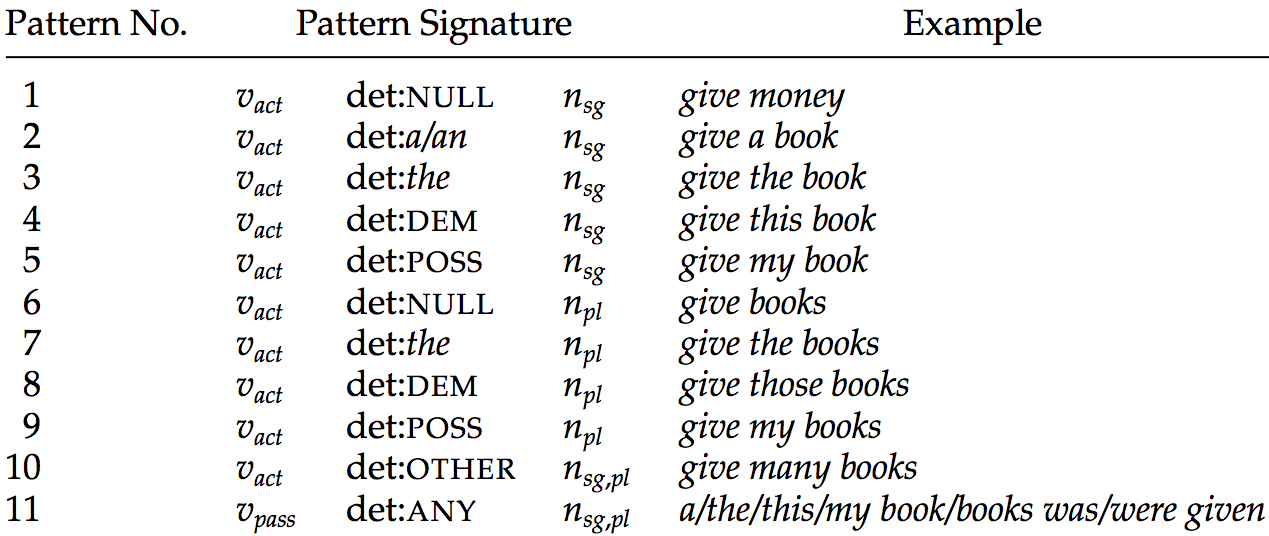
\includegraphics[width=\linewidth]{./patterns}
%%   \caption{List of patterns for VNC's.}
%%   \label{patterns}
%% \end{figure}

%% %Waseem paper
%% The closest work to ours is the work done in \cite{gharbieh2016word},
%% where they also apply word embeddings to identify idiomaticity of an
%% VNC. They represent an instance of an VNC by first averaging the two
%% word embeddings for the lemmas of the two components in the VNC to
%% form the vector $t$. They then average the embeddings of the context
%% words within a predetermined window separately for the verb and noun
%% giving the vectors $v$ and $n$, respectively. The vectors $v$ and $n$
%% are then averaged forming $vn$. They generate their final feature
%% vector by subtracting $vn$ from $t$ and concatenating it with a binary
%% feature representing if the instances is in a canonical form. They
%% proposed a supervised and unsupervised model, which both use the same
%% feature vector that was described above. Their supervised model uses
%% an SVM for classification. Their unsupervised model uses k-means
%% clustering to form clusters and they label the instances in a cluster
%% idiomatic if the majority of them are in a canonical form.


%% %The Salton et al. description
%% \cite{salton-ross-kelleher} used instances from the dataset used in
%% the experiments of \cite{Cook2008}, which is the same dataset that we
%% used and describe in Section
%% \ref{dataset}. \cite{salton-ross-kelleher} generate a training a
%% testing set by preserving a distribution over a number of idiomatic
%% and literal usages of an VNC. Each VNC will be in both the training
%% and testing allowing a model to see each VNC that is in the testing
%% while training on the training set. They represent an instance of an
%% VNC by embedding the sentence that it occurs in using the
%% skip-thoughts model, which embeds a sentence using an autoencoder. The
%% embedding of the sentence is then used as input to an SVM. They use
%% two different setups --a per expression setup and a general setup. The
%% per expression setup contains an SVM trained on a VNC and only
%% classifies instances containing the same VNC. The general setups
%% contains an SVM that is trained on all instances in the training set
%% regardless of which VNC is present. For both the per expression setup
%% and the general setup, they compared the performance of three
%% different types of SVM's including a linear SVM, a linear SVM that
%% used stochastic gradient descent, and an SVM with a polynomial
%% kernel. They also used a k-nearest neighbour classifier for the per
%% expression setup as well, where they evaluated their model with
%% different values for k. The per expression setup was only used on four
%% VNC's --blow\_whistle, lose\_head, make\_scene, and take\_heart. They
%% averaged the recall, precision, and f1-score over ten runs. The linear
%% SVM and the SVM with a polynomial kernel achieved the highest f1-score
%% overall in the general setup. The SVM with polynomial kernel achieved
%% the highest f1-score on most of the VNC's in the per expression setup.

\section{Models}\label{models}

%% In this section, we describe each model that we use to represent VNC
%% token instances. For each model, a linear SVM classifier is trained on
%% these representations.

We describe the models used to represent VNC token instances
below. For each model, a linear SVM classifier is trained on these
representations.


%Describes the embeddings models (not how they are applied)
\subsection{Word2vec}\label{word2vec}
%
%The word2vec model of \newcite{mikolov+:2013a} uses a feed forward
%artificial neural network to generate word embeddings. There are two
%methods in the word2vec framework --- skip-gram and continuous
%bag-of-words (CBOW). The skip-gram model is given a target word as
%input, and predicts the words surrounding the target word within a
%window of pre-determined size. This window slides across running text
%as the network updates its weights to learn embeddings representing
%each word in the vocabulary. The CBOW model is similar to the
%skip-gram model, except that it uses the context words as input and
%predicts the target word. In this paper we use skip-gram, because it
%often performs better than CBOW on tasks involving semantics \citep{mikolov+:2013a}.
%

We trained word2vec's skip-gram model \citep{mikolov+:2013b} on a
snapshot of Wikipedia from September 2015, which consists of
approximately 2.6 billion tokens. We used a window size of $\pm$8 and
300 dimensions. We ignore all words that occur less than fifteen times
in the training corpus, and did not set a maximum vocabulary size. We
perform negative sampling and set the number of training epochs to
five. We used batch processing with approximately 10$k$ words in each
batch.
	
%% TODO: Work in a note that this normalization is what fasttext does to
%% use word embeddings to represent a sentence

To embed a given a sentence containing a VNC token instance, we
average the word embeddings for each word in the sentence, including
stopwords.\footnote{Preliminary experiments showed that models
  performed better when stopword removal was not applied.} Prior to
averaging, we normalize each embedding to have unit length.

%% We looked at two different setups with one being that we
%% normalize each word embedding to be mapped onto a $n$-dimensional
%% sphere, which makes all vectors have a unit length of one. The average
%% vector is then used as input to an SVM used for classification.
% \url{http://www.lextek.com/manuals/onix/stopwords1.html}
\subsection{Siamese CBOW}

%The Siamese CBOW model \cite{kenter-borisov-derijke} learns word
%embeddings that are better able to represent a sentence through
%averaging than conventional word embeddings learned through skip-gram
%or CBOW. During training, this model averages the word embeddings in a
%target sentence, as well as the sentence before and after the
%target. The model then updates the word embeddings such that the
%sentences surrounding the target sentence have high probability given
%the target sentence, based on cosine similarity between two sentence
%vectors.

The Siamese CBOW model \cite{kenter-borisov-derijke} learns word
embeddings that are better able to represent a sentence through
averaging than conventional word embeddings such as skip-gram or
CBOW. We use a Siamese CBOW model that was pretrained on a snapshot of
Wikipedia from November 2012 using randomly initialized word
embeddings.\footnote{\url{https://bitbucket.org/TomKenter/siamese-cbow}}
Similarly to the word2vec model, to embed a given sentence containing
a VNC instance, we average the word embeddings for each word in the
sentence.

%% , excluding stopwords.

%% Put this back if you did exclude stopwords.


%% The average vector is then again used as input to a linear SVM for
%% classification.


\subsection{Skip-thoughts}
%
%Unlike the previous two models, skip-thoughts \citep{Kiros+:2015}
%generates embeddings for sentences directly, as opposed to via
%averaging of word embeddings. This model uses an autoencoder, which
%has one encoder --- a recurrent neural network --- to encode a target
%sentence, and two decoders --- also recurrent neural networks --- to
%generate the sentences before and after the target sentence given the
%output of the encoder. The weights of the encoder and decoders are
%trained and updated together. Once the model is trained, it represents
%a sentence by passing it through the encoder (and the decoder is not
%used at this stage).

%% Skip-thoughts \citep{Kiros+:2015} uses an autoencoder to generate an
%% embedding of a sentence. 

We use a publicly-available skip-thoughts model, that was pre-trained
on a corpus of
books.\footnote{\url{https://github.com/ryankiros/skip-thoughts}} We
represent a given sentence containing a VNC instance using the
skip-thoughts encoder.
%% \footnote{Unlike the previous two approaches, we
%%   do not remove stopwords here because this was not done when training
%%   the skip-thoughts model.}
%% As for the previous two approaches,
%% the embedding for the sentence is then used as input to a linear SVM
%% for classification.
Note that this approach is our re-implementation of the skip-thoughts
based method of \newcite{salton-ross-kelleher}, and we use it as a
strong baseline for comparison.


%% We embed a sentence differently compared to how we use word
%% embeddings. skip-thoughts embeds a sentence by inputting one word at a
%% time into the model in sequential order. The model then embeds the
%% sentence using the encoder. We do not remove stopwords in this case
%% because we want to preserve the word order. The encoding produced by
%% the model is used as input in an SVM for classification.

%
%
%\subsection{fastText}
%
%VNC token classification can be viewed as a document classification
%problem, in which sentences containing a VNC instance are (short)
%documents. \newcite{joulin-EtAl} propose fastText, a linear classifier
%in which documents are represented based on the average of their word
%embeddings. In this model, the word embeddings are randomly
%initialized, and updated during training of the classifier; i.e., word
%embeddings are learned for the specific classification
%task. \citeauthor{joulin-EtAl} found fastText to be a strong, and very
%fast, baseline for document classification that is competitive with
%more sophisticated deep learning approaches.
%
%We train fastText on ``documents'' corresponding to sentences
%containing VNC token instances, labelled with gold-standard judgements
%as to whether they are idiomatic or literal usages. In contrast to the
%previous approaches, this method using fastText does not require
%external resources (i.e., Wikipedia in the case of word2vec and
%Siamese CBOW, and the BookCorpus for skip-thoughts).

%% The fasttext model from \cite{joulin-EtAl} is trained with a task in
%% mind. 

%% It is trained by predicting a class when given a set of words. 

%% The embeddings of the words are averaged and then this average is used
%% in a linear regression algorithm to predict a class. 

%% The embeddings are updated as the model tries to predict a class for
%% the set of words. 

%% For example, we will be giving the model a sentence that contains an
%% VNC as input and it will predict if the sentence with the VNC belongs
%% to the idiom or literal class. 

%% The weights for the model are randomly initialized. 

%% This model does not require training on any external data like the
%% three models explained earlier. 

%% The word embeddings are initialized with randomly generated word
%% embeddings and then trained on our VNC dataset.



%% FastText is different from the other models that were discussed
%% because it is jointly trained with a linear regression algorithm. 

%% The model is given all the words as input, which then embeds the
%% sentence through averaging word embeddings and passes the average it
%% to its linear regressor to classify the instance.
%
%\subsection{Convolutional neural network}
%
%Convolutional neural networks (CNNs) are powerful classifiers that
%have been applied to achieve state-of-the-art results on broad
%coverage MWE identification \citep{gharbieh+:2017}. We therefore
%hypothesize that a a CNN might be particularly well-suited to the task
%of VNC token classification.
%
%The CNN that we use is based off of the one described in
%\cite{kim:2014}, but slightly simplified in that our model does not
%constrain the $l_2$ norms of the weight vectors in the output
%layer.\footnote{\url{https://github.com/dennybritz/cnn-text-classification-tf}}
%This model takes in a sentence as input, and maps each word to its
%embedding. These embeddings can be randomly initialized, or
%pre-trained embeddings (e.g., from word2vec). The model then applies
%filters over the word embeddings, which are functions that sum over
%the multiplication of their weight matrices with the word
%embeddings. There can be multiple filters of different sizes. The
%filter size determines how many words a filter sees at one time. To
%form the convolutional layer, the filters move across the entire
%sentence performing their matrix multiplication and summation at each
%step. The output is then given to the max-pooling layer, where the
%maximum value produced by each filter is taken and concatenated
%together. Finally, the concatenated vector is used as a feature vector
%to calculate the probability of each class (in our case, literal and
%idiomatic) using softmax.
%
%We consider two variants of this CNN, using different approaches to
%initialize the word embeddings. In the first case, the word embeddings
%are randomly initialized. For the second approach, we use pre-trained
%word embeddings from word2vec; here the embeddings used are the same
%as those described in section \ref{word2vec}. Using word embeddings to
%initialize the weights have been shown to increase the performance on
%text classification \citep{kim:2014}.


\section{Data and evaluation}


In this section, we discuss the dataset used in our experiments, and
the evaluation of our models.

\subsection{Dataset}\label{dataset}

We use the VNC-Tokens dataset \citep{Cook2008} --- the same dataset
used by \newcite{Fazly2009} and \newcite{salton-ross-kelleher} --- to
train and evaluate our models. This dataset consists of sentences
containing VNC usages drawn from the British National Corpus
\citep{Burnard2000},\footnote{\url{http://www.natcorp.ox.ac.uk}} along
with a label indicating whether the VNC is an idiomatic or literal
usage (or whether this cannot be determined, in which case it is
labelled ``unknown''). 

%% This is the same dataset used by
%% \newcite{Fazly2009} and \newcite{salton-ross-kelleher}.


VNC-Tokens is divided into \dev and \test sets that each include
fourteen VNC types and a total of roughly six hundred instances of
these types annotated as literal or idiomatic. Following
\newcite{salton-ross-kelleher}, we use \dev and \test, and ignore all
token instances annotated as ``unknown''.


%% VNC-Tokens consists of a total of roughly three thousand token
%% instances of fifty-three VNC types. Following
%% \newcite{salton-ross-kelleher}, we used two portions of the divided
%% dataset from \newcite{Cook2008}, \dev and \test, and ignore all token
%% instances annotated as ``unknown''. \newcite{Fazly2009} also carried
%% out experiments on this portion of the dataset. \dev and \test each
%% include fourteen VNC types, and a total of roughly six hundred
%% instances of these types annotated as literal or idiomatic.

%% The dataset that we worked with was from the corpus of VNC used in
%% \cite{Cook2008}, which was also used by \cite{salton-ross-kelleher}
%% and \cite{Fazly2009}. 



%% Both \cite{salton-ross-kelleher} and \cite{Fazly2009} used a different
%% distribution of VNC's for their
%% evaluation. 

\newcite{Fazly2009} and \newcite{salton-ross-kelleher} structured
their experiments differently. \citeauthor{Fazly2009} report results
over \dev and \test separately. In this setup
\test consists of expressions that were not seen during model
development (done on \dev). \citeauthor{salton-ross-kelleher},
on the other hand, merge \dev and \test, and create
new training and testing sets, such that each expression is present in
the training and testing data, and the ratio of idiomatic to literal
usages of each expression in the training data is roughly equal to
that in the testing data.

%% \cite{salton-ross-kelleher} distributed the dataset so that there were
%% instances of each VNC in both the training and testing set.  This
%% ensures that a model has seen each VNC during training. They also used
%% a predetermined number of idiom instances and literal instances that
%% are in the training and testing set for each VNC. Again, this ensures
%% a model has seen both usages of each VNC during training.

%% \cite{Fazly2009} separates the training and testing set
%% based on the VNC's in a way that the same VNC is not in both sets. For
%% example, all instances of a single VNC will be in either the training
%% set or the testing set but not both of them. 

We borrowed ideas from both of these approaches in structuring our
experiments. We retain the type-level division of 
%% \newcite{Cook2008} and 
\newcite{Fazly2009} into \dev and \test. We then divide each of
these into training and testing sets, using the same ratios of
idiomatic to literal usages for each expression as
\newcite{salton-ross-kelleher}.
%% Both \dev and \test contain fourteen different VNCs. \dev consists
%% of 270 idiomatic, and 179 literal, usages in the training set, and
%% 92 idiomatic, and 53 literal, usages in the testing set. \test
%% consists of 298 idiomatic, and 172 literal, usages in the training
%% set, and 90 idiomatic, and 53 literal, usages in the testing set.
This allows us to develop and tune a model on \dev, and then determine
whether, when retrained on instances of unseen VNCs in (the training
portion of) \test, that model is able to generalize to new VNCs
without further tuning to the specific expressions in \test.

%% TODO: Add a fn that parameter tuning is quite expensive for the CNN,
%% so that motivates the division into dev and test that we look at.

%% \footnote{This is particularly desirable for our approach based on a
%%   CNN, where tuning the various parameters of this model is
%%   computationally expensive, and parameter settings would ideally .}

%
%\begin{table}
%\small
%\begin{center}
%\setlength{\tabcolsep}{5pt}
%\begin{tabular}{cccccc}
%\multirow{2}{*}{Dataset} & \multirow{2}{*}{Expression} & \multicolumn{2}{c}{Training} & \multicolumn{2}{c}{Testing} \\
%&  & \# Lit & \# Idm & \# Lit & \# Idm\\
%\hline
%\multirow{14}{*}{\textsc{dev}}
%& blow\_trumpet &7 &14 &3 &5\\
%& find\_foot &3 & 36 &2 &12\\
%& get\_nod & 2 & 17 &1 &6\\
%& hit\_road &5 &19 &2 &6\\
%& hit\_roof & 5 & 9 &2 &2\\
%& kick\_heel & 7 & 23 &1 &8\\
%& lose\_head & 14 &15 &5 &6\\
%& make\_face & 10 & 21 &4 &6\\
%& make\_pile & 12 & 6 &5 &2\\
%& pull\_leg &32 &8 &8 &3\\
%& pull\_plug &16 &34 &4 &11\\
%& pull\_weight &4 &20 &2 &7\\
%& see\_star &46 & 3 &10 &2\\
%& take\_heart & 16 & 45 &4 &16\\
%\cline{2-6}
%& Total & 197 &270 &53 &92\\
%\hline
%\multirow{14}{*}{\textsc{test}}
%& blow\_top & 3 & 18 &2 &5 \\
%& blow\_whistle &39 &20 &12 &7 \\
%& cut\_figure & 5 & 28 &2 &8 \\
%& get\_sack & 34 & 6 &1 &9 \\
%& get\_wind &12 &9 &4 &4 \\
%& have\_word &8 &61 &3 &19 \\
%& hit\_wall &44 &6 &12 &1 \\
%& hold\_fire &14 &5 &2 &2 \\
%& lose\_thread & 1 &15 &1 &3 \\
%& make\_hay &6 & 6 &2 &3 \\
%& make\_hit &6 &3 &3 &2 \\
%& make\_mark &10 &56 &3 &16 \\
%& make\_scene &15 &22 &5 &8 \\
%& pull\_punch &3 &15 &1 &3 \\
%\cline{2-6}
%&Total &172 &298 &53 &90 \\
%\hline
%%\hline
%\end{tabular}
%\caption{The number of literal (Lit) and idiomatic (Idm) token
%  instances of each VNC expression in the training and testing
%  portions of \dev and \test.\label{detailDataset}}
%\end{center}
%\end{table}



%% The numbers reported above for the size of the dataset exactly match
%% the numbers reported in Cook et al. 2008

%% The CNN model uses a softmax algorithm to perform its prediction. It
%% is given all the words in a sentence as input. These words are then
%% mapped to their word embeddings, which is either randomly initialized
%% or initialized with word embeddings. The embeddings then go through a
%% convolutional layer and a max-pooling layer that were discussed in
%% Section \ref{models}. The model then concatenates the outputs of the
%% max-pooling layer, which is then used to make a prediction based on a
%% softmax algorithm.

\subsection{Evaluation}\label{eval}

The proportion of idiomatic usages in the testing portions of both
\dev and \test is 63\%. We therefore use accuracy to evaluate our
%% models following \cite{Fazly2009} because the classes (idiomatic and
%% literal) are roughly balanced.  Following
models following \newcite{Fazly2009} because the classes are roughly
balanced.  
%% Following \newcite{salton-ross-kelleher}, we randomly divide both \dev
%% and \test into training and testing portions ten times, and report
%% results as the average accuracy over these. To compute the accuracy
%% for a given run, we calculate the accuracy for each expression, and
%% then compute the average accuracy over these expressions.
We randomly divide both \dev and \test into training and testing
portions ten times, following \newcite{salton-ross-kelleher}. For each
of the ten runs, we compute the accuracy for each expression, and then
compute the average accuracy over the expressions. We then report
the average accuracy over the ten runs.



%% Old bits
%% Each model is applied ten times with instances shuffling between the
%% training and testing set each time. An average of the accuracy for the
%% ten runs is calculated as the performance of the model. The accuracy
%% is a fair evaluation in this model because the distribution over
%% classes does not greatly favor one class over the other. For example,
%% a strong accuracy on a set with the distribution of 80 idiom instances
%% and 10 literal instances may not represent how well a model performs
%% on the literal class, even if the model classified all literal
%% instances incorrect. Our datasets consists 64\% and 63\% idiomatic on
%% the Dev and Test set respectively, which shows a slight bias towards
%% the idiom class but this bias is present in real text written by
%% people \citep{Fazly2009}.


%\subsection{Embedding an Instance}\label{applied}
%Specifics about the embeddings that are used in the experiment

%Word2vec
%Given a sentence with a VNC, the word2vec model averages the word embeddings for each of the words in the sentence excluding stopwords\footnote{\url{http://www.lextek.com/manuals/onix/stopwords1.html}}. Stopwords are common words that are common in a language and therefore can create biases that hinder the performance of a text classification model. We looked at two different setups with one being that we normalize each word embedding to be mapped onto a $n$-dimensional sphere, which makes all vectors have a unit length of one. The average vector is then used as input to an SVM used for classification. 
%Siamese
%The Siamese CBOW model was specifically trained to represent a sentence by averaging its word embeddings. We embed an instance with the siamese CBOW model using the same technique as the word2vec model. The word embeddings are averaged excluding stopwords. We also use this model with and without normalizing the individual word embeddings. Again, we input the average vector into an SVM for classification.

%Skip-thoughts
%Unlike the first two embeddings, skip-thoughts embeds a sentence by inputting one word at a time into the model in sequential order. The model then embeds the sentence using the encoder. We do not remove stopwords in this case because we want to preserve the word order. The encoding produced by the model is used as input in an SVM for classification.

%FastText
%FastText is different from the other models that were discussed because it is jointly trained with an SVM. The model is given all the words as input, which then embeds the sentence through averaginf word embeddings and passes it to its SVM to classify the instance.

%CNN
%The CNN model does not use an SVM as a classifier because it is a classifier. It is given all the words in a sentence as input. These words are then mapped to their word embeddings, which is either randomly initialized or initialized with word embeddings. The embeddings then go through a convolutional layer and a max-pooling layer that were discussed in Section \ref{models}. The model then concatenates the outputs of the max-pooling layer, which is then used to make a prediction based on a softmax method.

\section{Experimental results}

In this section we first consider the effect of tuning the cost
parameter of the SVM for each model on \dev, and then report results
on \dev and \test using the tuned models.

%% old bits
%% will look at and discuss the performance of the
%% models during tuning as well as their performance on each dataset. We
%% compare using three different types of features including: only the
%% embeddings, embeddings with the pattern identified, and embeddings
%% with the canonical form being labeled as present or not.

\begin{table}
\setlength{\tabcolsep}{0.17em}
\begin{center}
\begin{tabular}{l|ccccc}
\multirow{2}{*}{Model} & \multicolumn{5}{c}{Penalty cost}\\
\cline{2-6}
 &0.01 &0.1 &1 &10 &100\\
\hline
%% Word2vec  &0.619 &0.649 &0.798 &\textbf{0.825} &0.805 &0.776\\
Word2vec     &0.619 &0.654 &0.818 &\textbf{0.830} &0.807\\
Siamese CBOW &0.619 &0.621 &0.665 &0.729 & \textbf{0.763}\\
%% Siamese CBOW(N) &0.619 &0.619 &0.645 &0.720 & 0.738 &\textbf{0.746}\\
Skip-thoughts &0.661& 0.784 &\textbf{0.803} &0.800 &0.798\\
\end{tabular}
\caption{Accuracy on \dev while tuning the penalty cost for the SVM
  for each model. The highest accuracy for each model is shown in
  boldface. \label{TuningAll}}
\end{center}
\end{table}



%\begin{table*}
%\begin{center}
%\begin{tabular}{l|cccccc}
%\multirow{2}{*}{Model} & \multicolumn{6}{c}{Penalty cost}\\
%\cline{2-7}
% &0.001 &0.01 &0.1 &1 &10 &100\\
%\hline
%%% Word2vec  &0.619 &0.649 &0.798 &\textbf{0.825} &0.805 &0.776\\
%Word2vec     &0.619 &0.619 &0.654 &0.818 &\textbf{0.830} &0.807\\
%Siamese CBOW &0.619 &0.619 &0.621 &0.665 &0.729 & \textbf{0.763}\\
%%% Siamese CBOW(N) &0.619 &0.619 &0.645 &0.720 & 0.738 &\textbf{0.746}\\
%Skip-thoughts &0.619 &0.661& 0.784 &\textbf{0.803} &0.800 &0.798\\
%\end{tabular}
%\caption{Accuracy on \dev while tuning the penalty cost for the SVM
%  for each model. The highest accuracy for each model is shown in
%  boldface. \label{TuningAll}}
%\end{center}
%\end{table*}


%
%\begin{table}
%\begin{center}
%\begin{tabular}{l|c}
%Parameter & Default setting \\
%\hline
%Filter size & 3,4,5 \\
%Number of filters & 128 \\
%Number of epochs & 200\\
%Embedding size & 200\\
%\end{tabular}
%\caption{Default parameter settings for tuning the CNN
%  models.\label{defaultVals}}
%\end{center}
%\end{table}


\subsection{Parameter tuning}

%We will discuss the tuning of the penalty cost for the linear SVM that is
%used by several models. The parameter tuning is carried out on \dev. 
%We then discuss tuning parameters for the CNN models. All of this parameter tuning is carried out on \dev.

We tune the SVM for each model on \dev by carrying out a linear search
for the penalty cost from $0.01$--$100$, increasing by a factor of ten
each time. Results for this parameter tuning are shown in
\tabref{TuningAll}. These results highlight the importance of choosing
an appropriate setting for the penalty cost. For example, the accuracy
of the word2vec model ranges from $0.619$--$0.830$ depending on the
cost setting. In subsequent experiments, for each model, we use the
penalty cost that achieves the highest accuracy in \tabref{TuningAll}.

%The process for tuning the parameters of the CNN models is
%substantially more involved, due to the number of different parameters
%to consider. There are four parameters that we tune: the filter size,
%number of filters, number of epochs, and embedding size. The default
%settings we choose for these parameters are shown in
%\tabref{defaultVals}.
%
%The filter size determines how many words a filter sees. Filters of
%multiple sizes can be used at once. For example, the default number of
%filters of $3,4,5$ indicates that there are $n$ filters of size $3$,
%$n$ filters of size $4$, and $n$ filters of size $5$, where $n$ the
%number of filters parameter. The number of epochs is the number of
%training epochs (i.e., iterations over the training data). Finally,
%the embedding size is the size of the word embeddings in the lookup
%table. We consider variants of the CNN model with randomly initialized
%embeddings, and embeddings initialized from word2vec embeddings,
%referred to as CNN-random and CNN-word2vec, respectively. This tuning
%of the embedding size only applies to CNN-random; for CNN-word2vec we
%only consider the 300 dimensional embeddings described in
%\secref{word2vec}.
%
%We tuned each parameter separately, while leaving all other parameters
%constant at their default values. Specifically we consider the ranges
%of parameter values indicated in \tabref{TuningCNN}.\footnote{Due to
%  the number of parameters, considering all parameter setting
%  combinations was not feasible due to the computational cost.} We
%then trained CNN-random and CNN-word2vec using the combination of
%parameter settings found to perform best when tuned individually. In
%both cases this led to lower accuracy compared to the best results in
%\tabref{TuningCNN} for each model. We therefore use the best parameter
%settings found in \tabref{TuningCNN}. In subsequent experiments,
%CNN-random uses 128 filters of sizes 2,3,4, an embedding size of 200,
%and is trained for 200 epochs. CNN-word2vec uses 128 filters of
%sizes 3,4,5, an embedding size of 300, and is trained for 500 epochs.




%% The default value for each parameter are given in Table
%% \ref{defaultVals}. We trained two CNN models --one for regular CNN and
%% one for CNNw2v-- using the parameters that achieve the highest
%% accuracy. This resulted in a worse performance compared to the best
%% reported results for each model in the tuning, 
%Best paramters for CNNw2v: 0.80298
%Used default values with 500 dimensions for Test set
%
%\begin{table*}
%\begin{center}
%\begin{tabular}{llllll}
%Filter Size & 1 &1,2 & 2,3,4 &3,4,5 &1,2,3,4,5\\
%\hline
%CNN-random & 0.7462 &0.7643 & \textbf{\underline{0.7799}} &0.7655 &0.7470\\
%CNN-word2vec& 0.7864 &0.7880 &0.7938 &\textbf{0.8036} &0.8017\\
%~\\[-8pt]
%\# Filters &64 &128 &256 &512 &1024\\
%\hline
%CNN-random & 0.7575 &0.7655 &0.7590 & \textbf{0.7777} &0.7465\\
%CNN-word2vec& 0.7925 &0.8036 &0.7968 &0.8040 & \textbf{0.8041}\\
%~\\[-8pt]
%\# Epochs &100 &200 &300 &400 &500\\
%\hline
%CNN-random & 0.7639 &0.7655 &0.7693 &0.7526 & \textbf{0.7731}\\
%CNN-word2vec&0.7988 &0.8036 &0.8087 &0.8015 &\textbf{\underline{0.8109}}\\
%~\\[-8pt]
%Size & 100 &200 &300 &400 &500\\
%\hline
%CNN-random & 0.7516 &0.7655 &0.7576 &0.7702 & \textbf{0.7793}\\ 
%
%\end{tabular}
%\caption{Accuracy on \dev while tuning parameters for the CNN
%  models. For each model, the highest accuracy obtained when tuning
%  each parameter individually is shown in boldface. The highest
%  accuracy for each model is underlined.\label{TuningCNN}}
%\end{center}
%\end{table*}

%PC: Do we want to rotate this table?

%\multirow{2}{*}{Model} & \multicolumn{6}{c}{Penalty cost}\\
%\small
\begin{table}
\setlength{\tabcolsep}{0.4em}
\begin{center}
\begin{tabular}{l|cc|cc}
\multirow{2}{*}{Model}  &  \multicolumn{2}{c}{\dev}  &  \multicolumn{2}{c}{\test}\\
\cline{2-5}
& $-$CF & $+$CF & $-$CF & $+$CF\\
\hline
CForm & - & 0.721 & - & 0.749\\
Word2vec &\textbf{0.830} &\textbf{0.854}& \textbf{0.804} &\textbf{0.852}\\
Siamese CBOW &0.763 &0.774 & 0.717 &0.779\\
Skip-thoughts &0.803 &0.827& 0.786 &0.842\\
%FastText &0.7381 &0.7445\\
%CNN-random &0.7799 &0.7557\\
%CNN-word2vec &0.8109 & -\\
\end{tabular}
\caption{Accuracy on \dev and \test for each model, without ($-$CF)
  and with ($+$CF) the canonical form feature. The highest accuracy
  for each setting on each dataset is shown in
  boldface. \label{results}}
\end{center}
\end{table}

%
%\begin{table}
%\begin{center}
%\begin{tabular}{l|cc}
%Model & $-$CForm & $+$CForm \\
%\hline
%CForm         & - & 0.7488\\
%Word2vec      & \textbf{0.8036} &\textbf{0.8522}\\
%Siamese CBOW  & 0.7172 &0.7787\\
%Skip-thoughts & 0.7855 &0.8417\\
%%FastText      & 0.7484 &0.7601\\
%%CNN-random   & 0.7477 & 0.7302\\
%%CNN-word2vec & 0.7632 &-\\
%\hline
%\end{tabular}
%\caption{Accuracy on \test for each model, without ($-$CForm) and with
%  ($+$CForm) the canonical form feature. The highest accuracy for each
%  setting is shown in boldface. \label{TestResults}}
%\end{center}
%\end{table}
%
%
%\begin{table}
%\begin{center}
%\begin{tabular}{l|cc}
%Model  & $-$CForm & $+$CForm\\
%\hline
%CForm & - & 0.7207\\
%Word2vec &\textbf{0.8299} &\textbf{0.8537}\\
%Siamese CBOW &0.7633 &0.7740\\
%Skip-thoughts &0.8030 &0.8268\\
%%FastText &0.7381 &0.7445\\
%%CNN-random &0.7799 &0.7557\\
%%CNN-word2vec &0.8109 & -\\
%\end{tabular}
%\caption{Accuracy on \dev for each model, without ($-$CForm) and with
%  ($+$CForm) the canonical form feature. The highest accuracy for each
%  setting is shown in boldface. \label{DevResults}}
%\end{center}
%\end{table}

%% Old table

%% \begin{table}
%% \small
%% \begin{center}
%% \begin{tabular}{l|ccc}

%% &Basic
%% &Pattern
%% &Binary\\
%% \hline
%% Cform
%% &0.7207
%% &-
%% &-\\
%% Word2vec Not normalized
%% &0.8245
%% &\textbf{0.8172}
%% &\textbf{0.8559}\\
%% Word2vec Normalized
%% &\textbf{0.8299}
%% &0.8163
%% &0.8537\\
%% Siamese CBOW not normalized
%% &0.7633
%% &0.7623
%% &0.7740\\
%% Siamese CBOW normalized
%% &0.7459
%% &0.7564
%% &0.7671\\
%% Skip-thoughts
%% &0.8030
%% &0.8030
%% &0.8268\\
%% FastText
%% &0.7381
%% &0.7401
%% &0.7445\\
%% CNN
%% &0.7799
%% &0.7346
%% &0.7557\\
%% CNNword2vec
%% &0.8008
%% &-
%% & -\\

%% \hline
%% \end{tabular}
%% \caption{Accuracy on the Dev set with the highest accuracy for each feature being in bold. \label{DevResults}}
%% \end{center}
%% \end{table}


\subsection{\dev and \test results}

%% In \tabref{results} we report results on \dev and \test for each model,
%% %% described in \secref{models}
%% as well as the unsupervised CForm model of \newcite{Fazly2009},
%% %% (see \secref{related})
%% which simply labels a VNC as idiomatic if it occurs in its canonical
%% form, and as literal otherwise. We further consider each model (other
%% than CForm) in two setups, $-$CF and $+$CF.  The $-$CF setup
%% corresponds to the models as described in \secref{models}. The $+$CF
%% setup further incorporates lexico-syntactic knowledge of canonical
%% forms into each model by concatenating the embedding representing each
%% VNC token instance with a one-dimensional vector which is one if the
%% VNC occurs in a canonical form, and zero otherwise.

In \tabref{results} we report results on \dev and \test for each
model,
%% described in \secref{models}
as well as the unsupervised CForm model of \newcite{Fazly2009},
%% (see \secref{related})
which simply labels a VNC as idiomatic if it occurs in its canonical
form, and as literal otherwise. We further consider each model (other
than CForm) in two setups.  $-$CF corresponds to the models as
described in \secref{models}. $+$CF further incorporates
lexico-syntactic knowledge of canonical forms into each model by
concatenating the embedding representing each VNC token instance with
a one-dimensional vector which is one if the VNC occurs in its
canonical form, and zero otherwise.

We first consider results for the $-$CF setup. On both \dev and \test,
the accuracy achieved by each supervised model is higher than that of
the unsupervised CForm approach, except for Siamese CBOW on \test. The
word2vec model achieves the highest accuracy on \dev and \test of
$0.830$ and $0.804$, respectively. The difference between the word2vec
model and the next-best model, skip-thoughts, is significant using a
bootstrap test \cite{Berg-Kirkpatrick+:2012} with 10$k$ repetitions
for \dev ($p=0.006$), but not for \test ($p=0.051$). Nevertheless, it
is remarkable that the relatively simple approach to averaging word
embeddings used by word2vec performs as well as, or better than, the
much more complex skip-thoughts model used by
\newcite{salton-ross-kelleher}.\footnote{The word2vec and
  skip-thoughts models were trained on different corpora, which could
  contribute to the differences in results for these models. We
  therefore carried out an additional experiment in which we trained
  word2vec on BookCorpus, the corpus on which skip-thoughts was
  trained. This new word2vec model achieved accuracies of 0.825 and
  0.809, on \dev and \test, respectively, which are also higher
  accuracies than those obtained by the skip-thoughts model.}

Turning to the $+$CF setup, we observe that, for both \dev and \test,
each model achieves higher accuracy than in the $-$CF
setup.\footnote{In order to determine that this improvement is due to
  the information about canonical forms carried by the additional
  feature in the $+$CF setup, and not due to the increase in number of
  dimensions, we performed additional experiments in which we
  concatenated the embedding representations with a random binary
  feature, and with a randomly chosen value between $0$ and $1$. For
  each model, neither of these approaches outperformed that model
  using the $+$CF setup.}  All of these differences are significant
using a bootstrap test ($p<0.002$ in each case). In addition, each
method outperforms the unsupervised CForm approach on both \dev and
\test. These findings demonstrate that the linguistically-motivated,
lexico-syntactic knowledge encoded by the canonical form feature is
complementary to the information from a wide range of types of
distributed representations. In the $+$CF setup, the word2vec model
again achieves the highest accuracy on both \dev and \test of $0.854$
and $0.852$, respectively.\footnote{In the $+$CF setup, the word2vec
  model using embeddings that were trained on the same corpus as
  skip-thoughts achieved accuracies of 0.846 and 0.851, on \dev and
  \test, respectively. These are again higher accuracies than the
  corresponding setup for the skip-thoughts model.}  The difference
between the word2vec model and the next-best model, again
skip-thoughts, is significant for both \dev and \test using a
bootstrap test ($p<0.05$ in each case).

 \begin{table*}
 \begin{center}
 \begin{tabular}{cccccccccc}
\multirow{2}{*}{Model} &\multicolumn{3}{c}{Idiomatic} & &
\multicolumn{3}{c}{Literal} & & \multirow{2}{*}{Ave. F} \\ 

\cline{2-4} \cline{6-8} &P & R & F & &P & R & F & & \\ \hline

CForm&0.766& 0.901 &0.794& & 0.668&0.587&0.576& & 0.685 \\

Word2vec $-$CF &0.815&0.879&0.830&& 0.627&0.542&0.556&& 0.693\\

Word2vec $+$CF& 0.830 &0.892& 0.848 & & 0.758 & 0.676 & 0.691 & & 0.770\\
 \end{tabular}
 \caption{Precision (P), recall (R), and F1 score (F), for the
   idiomatic and literal classes, as well as average F1 score
   (Ave. F), for \test.\label{posneg}}
 \end{center}
 \end{table*}

To better understand the impact of the canonical form feature when
combined with the word2vec model, we compute the average precision,
recall, and F1 score for each MWE for both the positive (idiomatic)
and negative (literal) classes, for each run on \test.\footnote{We
  carried out the same analysis on \dev. The findings were similar.}
For a given run, we then compute the average precision, recall, and F1
score across all MWEs, and then the average over all ten runs. We do
this using CForm, and the word2vec model with and without the
canonical form feature. Results are shown in \tabref{posneg}. In line
with the findings of \newcite{Fazly2009}, CForm achieves higher
precision and recall on idiomatic usages than literal ones. In
particular, the relatively low recall for the literal class indicates
that many literal usages occur in a canonical form. Comparing the
word2vec model with and without the canonical form feature, we see
that, when this feature is used, there is a relatively larger increase
in precision and recall (and F1 score) for the literal class, than for
the idiomatic class. This indicates that, although the canonical form
feature itself performs relatively poorly on literal usages, it
provides information that enables the word2vec model to better
identify literal usages.

%% When the canonical form feature is used,
%% we see a relatively larger increase in precision and recall (and F1
%% score) for the literal class, than for the idiomatic class, suggesting
%% that the canonical form feature provides information that allows this
%% model to better identify literal usages.







%%  \begin{table*}
%%  \small
%%  \begin{center}
%%  \begin{tabular}{C{1.8cm}|C{0.4cm}C{0.4cm}C{0.5cm}|C{0.4cm}C{0.4cm}C{0.5cm}|C{0.5cm}|C{0.4cm}C{0.4cm}C{0.5cm}|C{0.4cm}C{0.4cm}C{0.5cm}|C{0.4cm}C{0.5cm}}
%% \cline{2-15}
%% &\multicolumn{7}{c|}{\dev} & \multicolumn{7}{c|}{\test} \\
%% \cline{2-15}
%% &\multicolumn{3}{c|}{Positive} & \multicolumn{3}{c|}{Negative} & Avg. & \multicolumn{3}{c|}{Positive} & \multicolumn{3}{c|}{Negative} &  \multicolumn{1}{c|}{Avg.}\\
%% \cline{2-15}
%% &P & R & F  &P & R & F &Avg. F & P & R & F   & P & R & F & \multicolumn{1}{c|}{Avg. F} \\
%% \hline

%% \vspace{-0.4cm} Cform&0.703&0.830&0.736&0.596&0.500&0.576&0.656&0.766&\textbf{0.901}\textbf&0.794&0.668&0.587&0.576&  \multicolumn{1}{C{0.5cm}|}{0.685} \\
%% \vspace{-0.4cm}Word2vec-CF &0.797&\textbf{0.868}&0.821&0.708&0.636&0.556&0.689&0.815&0.879&0.830&0.627&0.542&0.556&\multicolumn{1}{C{0.5cm}|}{0.693}\\
%% Word2vec+CF&\textbf{0.823}&0.853&\textbf{0.826}&\textbf{0.756}&\textbf{0.707}&\textbf{0.692}&\textbf{0.759}&\textbf{0.830}&0.892&\textbf{0.848}&\textbf{0.758}&\textbf{0.676}&\textbf{0.691}&\multicolumn{1}{C{0.5cm}|}{\textbf{0.770}}\\
%%  \end{tabular}
%%  \caption{Positive and negative precision (P), recall (R), F-score (F), and average F-score on \dev and\test. \label{posNeg}}
%%  \end{center}
%%  \end{table*}



%% \subsection{\dev results}

%% %% TODO: Discuss dev and test results in the same subsection, because we
%% %% have about the same to say about each of thema

%% We first consider resuls on \dev. In \tabref{results} we report
%% results for each model described in \secref{models}, as well as the
%% unsupervised CForm model of \newcite{Fazly2009}, which simply labels a
%% VNC as idiomatic if it occurs in its canonical form, and as literal
%% otherwise. We further consider each model (other than CForm) in two
%% setups, $-$CForm and $+$CForm. The $-$CForm setup corresponds to the
%% models as described in \secref{models}. The $+$CForm setup further
%% incorporates lexico-syntactic knowledge of canonical forms into the
%% various models. For the word2vec, Siamese CBOW, and skip-thoughts
%% models, this is done by concatenating the sentence-level embedding
%% that these models form with a one-dimensional vector, which is one if
%% the VNC occurs in a canonical form, and zero otherwise. 

%% %\footnote{Note, however, that for CNN-word2vec,
%% %  this approach to incorporating knowledge of canonical forms cannot
%% %  be used. Tokens that are augmented in this way do not occur in the
%% %  word2vec vocabulary, because these embeddings were trained on an
%% %  external corpus (Wikipedia) that does not include annotations for
%% %  canonical forms of VNCs. We therefore do not report results for
%% %  CNN-word2vec in the $+$CForm setup. For CNN-random, on the other
%% %  hand, this is not an issue, because it builds its vocabulary by
%% %  first reading in all training instances, so it will have these
%% %  augmented tokens in its vocabulary.}


%% %% old bits
%% %% The first dataset that we explore is the Dev set as shown in Table
%% %% \ref{DevResults}. We compare all models in the three setups
%% %% --\textit{Basic, Pattern, Binary}. The \textit{Basic} setup does not
%% %% use any additional features with the embedding representations. The
%% %% \textit{Pattern} setup concatenates the embedding representation with
%% %% a pattern vector, which is one-hot vector with all zeros except a one
%% %% in the index related to the pattern identified. This process is done
%% %% for all models that do not jointly train their classifier with their
%% %% word embeddings such as the word2vec, siamese CBOW, and skip-thoughts
%% %% models. The training set for the fastText and CNN models is modified
%% %% so that the VNC is concatenated with its pattern number to make a new
%% %% word. This is done the same for the instances in the testing set as
%% %% well. Therefore, the model does not change, but rather the data itself
%% %% is altered. The similar processes are used for \textit{Binary}, where
%% %% the embedding of the sentence for the word2vec, siamese CBOW, and
%% %% skip-thoughts models are concatenated with a one-dimensional vector,
%% %% which is one if the VNC occurs in a canonical form and zero
%% %% otherwise. The fastText and CNN models again have the datasets altered
%% %% so that each VNC is concatenated with the word \textit{Canonical} if
%% %% the VNC occurs in the canonical form and \textit{NotCanonical}
%% %% otherwise. Looking at the results in Table \ref{DevResults}.

%% We begin by considering results for the $-$CForm setup. The accuracy
%% achieved by each supervised model is higher than that of the
%% unsupervised CForm model. The word2vec model achieves the highest
%% accuracy at $0.830$. Remarkably, the relatively simple approach to
%% averaging word embeddings used by word2vec outperforms the much more
%% complex skip-thoughts model used by
%% \newcite{salton-ross-kelleher}. 
%% %CNN-word2vec performs similarly to
%% %skip-thoughts, and outperforms CNN-random, which is inline with the
%% %findings of \newcite{kim:2014}. CNN-random, Siamese CBOW, and fastText
%% %achieve accuracies substantially lower than the other approaches.


%% %% The cform method, which simply labels a VNC as idiomatic if it occurs
%% %% in a canonical form \citep{Fazly2009}, is a simple baseline but
%% %% achieves similar results to siamese CBOW and fastText in the
%% %% \textit{Basic} setup. The word2vec-based models achieves the highest
%% %% accuracies under the \textit{Basic} setup with word2vec, that
%% %% normalizes its word embeddings, outperforming its non normalizing
%% %% counterpart with $0.8299$. Skip-thoughts and word2vec initialized CNN
%% %% achieve the next highest accuracies with $0.8030$ and $0.8008$,
%% %% respectively. The word2vec initialized CNN outperforms the CNN that
%% %% was randomly initialized, which supports the results of
%% %% \cite{kim:2014}. 

%% %% When we add the \textit{Pattern} feature, it hurts
%% %% the performance of four models and slightly increases or does not
%% %% change the performance for two models. Word2vec achieves the highest
%% %% accuracy under the \textit{Pattern} setup with an accuracy of
%% %% $0.8172$, only slightly increasing its performance. 

%% Turning to the $+$CForm setup, we observe that each model achieves higher accuracy than in the
%% $-$CForm setup. In addition, each method outperforms the unsupervised
%% CForm approach. These findings demonstrate that the
%% linguistically-motivated, lexico-syntactic knowledge encoded by the
%% canonical form feature is complementary to the information from a wide
%% range of types of distributed representations. In the $+$CForm setup,
%% the word2vec model again achieved the highest accuracy of
%% $0.854$. 
%% %Returning to the relatively poor performance of CNN-random
%% %in this setup, we note that the improvement here for fastText over the
%% %$-$CForm setup is also relatively small. Taken together, these
%% %findings suggest that the approach to incorporating knowledge of
%% %canonical forms into these models was less effective than the binary
%% %feature used in the other models which use an SVM.

%% %% TODO: Could comment that the ordering of the models in terms of
%% %% accuracy is the same in the -cform and +cform approaches.


%% %% Unlike the \textit{Pattern} feature, the \textit{Binary} feature
%% %% increases the performance of all models except one. The
%% %% \textit{Binary} hurts the CNN performance and only slightly increases
%% %% the fastText model, which might be due to the feature being added
%% %% differently with these models. It is not logical to use the
%% %% CNNword2vec in the same manner as CNN because the new tokens, that are
%% %% added with the identified pattern or presence of a canonical form,
%% %% would not be in the word2vec vocabulary and therefore would not add
%% %% any additional information. The CNN builds it vocabulary by first
%% %% reading in all training instances so it will have these new tokens in
%% %% its vocabulary. Word2vec achieves the highest accuracy under the
%% %% \textit{Binary} setup with $0.8599$. 

%% %% Each model under the \textit{Binary} setup outperforms their own
%% %% results under the \textit{Pattern} setup showing that the
%% %% \textit{Binary} feature is more valuable than the \textit{Pattern}
%% %% feature.


%% %\begin{table}
%% %\begin{center}
%% %\begin{tabular}{l|cc}
%% %Model & $-$CForm & $+$CForm \\
%% %\hline
%% %CForm         & - & 0.7488\\
%% %Word2vec      & \textbf{0.8036} &\textbf{0.8522}\\
%% %Siamese CBOW  & 0.7172 &0.7787\\
%% %Skip-thoughts & 0.7855 &0.8417\\
%% %%FastText      & 0.7484 &0.7601\\
%% %%CNN-random   & 0.7477 & 0.7302\\
%% %%CNN-word2vec & 0.7632 &-\\
%% %\hline
%% %\end{tabular}
%% %\caption{Accuracy on \test for each model, without ($-$CForm) and with
%% %  ($+$CForm) the canonical form feature. The highest accuracy for each
%% %  setting is shown in boldface. \label{TestResults}}
%% %\end{center}
%% %\end{table}

%% \subsection{\test results}

%% We now consider results on \test. Recall that this dataset consists of
%% VNC types that were not seen in \dev. Here we train on the training
%% portion of \test, and test on the testing portion of \test, but do not
%% perform any further tuning of our models. Results on \test for each
%% model, again in both the $-$CForm and $+$CForm setups, are shown in
%% \tabref{results}.

%% We again first consider the $-$CForm setup. In this case, the
%% word2vec and skip-thoughts models achieve higher
%% accuracies than the unsupervised CForm baseline, while the Siamese
%% CBOW model performs below this baseline. The
%% word2vec model again improves over the skip-thoughts model used by
%% \newcite{salton-ross-kelleher}, and again achieves the highest
%% accuracy (0.804).

%% Turning to the $+$CForm setup, we again see an improvement in the
%% accuracy for each model over its
%% accuracy in the $-$CForm setup. Moreover, although the Siamese CBOW
%% and fastText models performed below the unsupervised baseline in the
%% $-$CForm setup, in the $+$CForm setup, all models beat the unsupervised CForm baseline. This
%% finding further demonstrates the complementarity of the
%% lexico-syntactic knowledge carried by canonical forms, and the
%% information available in a variety of types of distributed
%% representations.


%% we see a similar story with the word2vec-based models achieving the
%% highest accuracies under all setups and the the \textit{Binary}
%% feature increases the performance of all models except the CNN
%% model. 

%% The one change with the results in this set is the effect that the
%% \textit{Pattern} has on the models. It increases the performance of
%% all models except fastText. Strangely, the CNN model with the
%% \textit{Pattern} feature outperforms the CNN with the \textit{Binary}
%% feature. An interesting note is that the only models that outperform
%% the cform baseline under the \textit{Basic} setup is the
%% word2vec-based models and the skip-thoughts model, which shows that
%% identifying the canonical forms of a VNC is a strong feature. The
%% word2vec initialized CNN no longer outperforms the randomly
%% initialized CNN but performs very similar.


\section{Conclusions}\label{conclusion}

%% Reiterate motivation for this work
Determining whether a usage of a VNC is idiomatic or literal is
important for applications such as machine translation, where it is
vital to preserve the meanings of word combinations. 
%% In this paper we considered the problem of classifying VNC token
%% instances as idiomatic or literal. We proposed two approaches to this
%% task based on word2vec embeddings and Siamese CBOW. 
In this paper we proposed two approaches to the task of classifying
VNC token instances as idiomatic or literal based on word2vec
embeddings and Siamese CBOW. We compared these approaches against a
linguistically-informed unsupervised baseline, and a model based on
skip-thoughts previously applied to this task
\citep{salton-ross-kelleher}. Our experimental results show that a
comparatively simple approach based on averaging word embeddings
performs at least as well as, or better than, the approach based on
skip-thoughts. We further proposed methods to combine linguistic
knowledge of the lexico-syntactic fixedness of VNCs --- so-called
``canonical forms'', which can be automatically acquired from corpora
via statistical methods --- with the embedding based approaches. Our
findings indicate that this rich linguistic knowledge is complementary
to that available in distributed representations.

%The CNN models did not improve when knowledge of canonical forms was
%included. In future work we therefore intend to consider alternative
%strategies to incorporating this information into the CNN
%models. 

Alternative approaches to embedding sentences containing VNC
instances could also be considered, for example, FastSent
\citep{Hill+:2016}. However, all of the models we used represent the
context of a VNC by the sentence in which it occurs. In future work we
therefore also intend to consider approaches such as context2vec
\citep{melamud2016context2vec} which explicitly encode the context in
which a token occurs. Finally, one known challenge of VNC token
classification is to develop models that are able to generalize to VNC
types that were not seen during training \citep{gharbieh+:2016}. In
future work we plan to explore this experimental setup.


%% Most models better their own performance when adding the
%% \textit{Binary} feature but is not the case for models whose added
%% this feature by changing the VNC in the text that the models train and
%% test on such as the fastText, and CNN models. This shows that a new
%% way to include this feature with these models is needed. The
%% \textit{Pattern} feature did not often increase the performance of
%% models and only increased the performance a small amount when it did
%% increase the performance of a model. This might be due to not enough
%% training data for each pattern. There are a possible eleven patterns
%% that VNC can belong to, which means their are fewer instances for each
%% pattern then there are for all the instances in the original
%% datasets. Regardless, it is not a valuable feature at the moment as it
%% was implemented, but leaves and interesting area to explore. The
%% patterns were useful for identifying canonical forms, which increased
%% the performance of most of our models.

% Future work

%% There are other models that generate embeddings of text that could be
%% applied to this task such as the context2vec model, which embed the
%% context of a target word \citep{melamud2016context2vec}. This model
%% could be used to embed the context of VNC since each VNC appears in
%% context. This model has been known to work well on other task that
%% require the representation of a word in context such as usage
%% similarity \citep{king-cook:2017}. As hinted at earlier, it would be
%% interesting to look more into the use of the \textit{Pattern} feature,
%% such as determine how well each model performs on each pattern. An
%% ensemble model could also be constructed where each model in the
%% ensemble is assigned a weight for each pattern, so their prediction
%% for an instance is weighted based on how well it can perform on the
%% pattern that is present in the instance. The issue with using the
%% \textit{Pattern} and \textit{Binary} with the fastText and CNN models
%% requires a new method to include these features. The architectures of
%% these models can be altered to allow the inclusion of a feature vector
%% to be concatenated to the vector that is used as input to their
%% classifier. This would be before the SVM in fastText, and before the
%% softmax in the CNN. The CNN that was initialized with word embeddings
%% could also be further explored by using different word embeddings for
%% initialization. The word2vec model could also use different word2vec
%% embeddings, such as embeddings that were trained on text that has the
%% pattern or the canonical forms identified. We do not specifically
%% capture much syntactic information --besides the pattern
%% identification-- with our models. Including syntactic information
%% might provide useful information similar to how it assisted models in
%% the PARSEME's verbal MWE identification task. In terms of the
%% classifiers, the SVM's that were used were trained on instances of
%% different VNC's and therefore are not specifically trained to identify
%% a single VNC. It is reasonable to assume that an SVM that is trained
%% on a specific VNC will outperform a more general model.

%\section*{Acknowledgments}

% include your own bib file like this:
%\bibliographystyle{acl}
%\bibliography{naaclhlt2018}
\bibliography{../bibtex/big}
\bibliographystyle{acl_natbib}


\end{document}
